\section{Results}
\label{sec:results}

\para{Base task performance.} The shared architecture reaches mean test accuracy $0.9270$ on \mnist, $0.8228$ on \fashionmnist, and $0.3937$ on \cifar, which establishes a simple but non-trivial benchmark across task difficulty. Best-seed performance follows the same ranking, with \mnist easiest and \cifar hardest.

\begin{figure}[t]
    \centering
    \begin{minipage}[t]{0.32\linewidth}
        \centering
        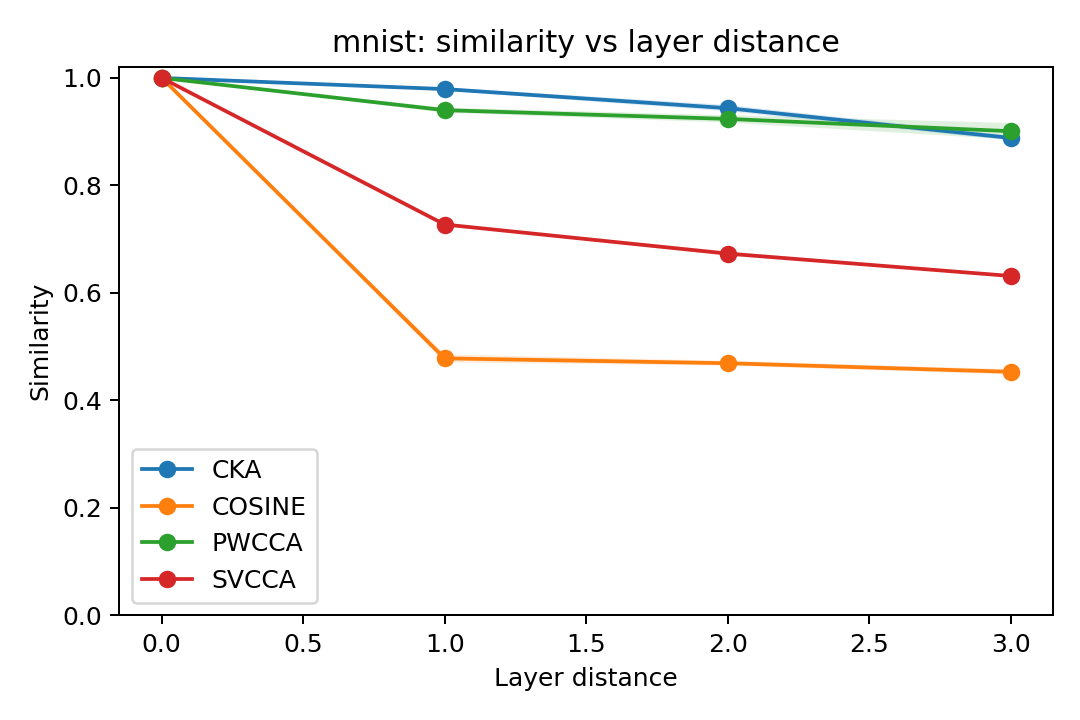
\includegraphics[width=\linewidth]{figures/mnist_distance_trend.png}
    \end{minipage}\hfill
    \begin{minipage}[t]{0.32\linewidth}
        \centering
        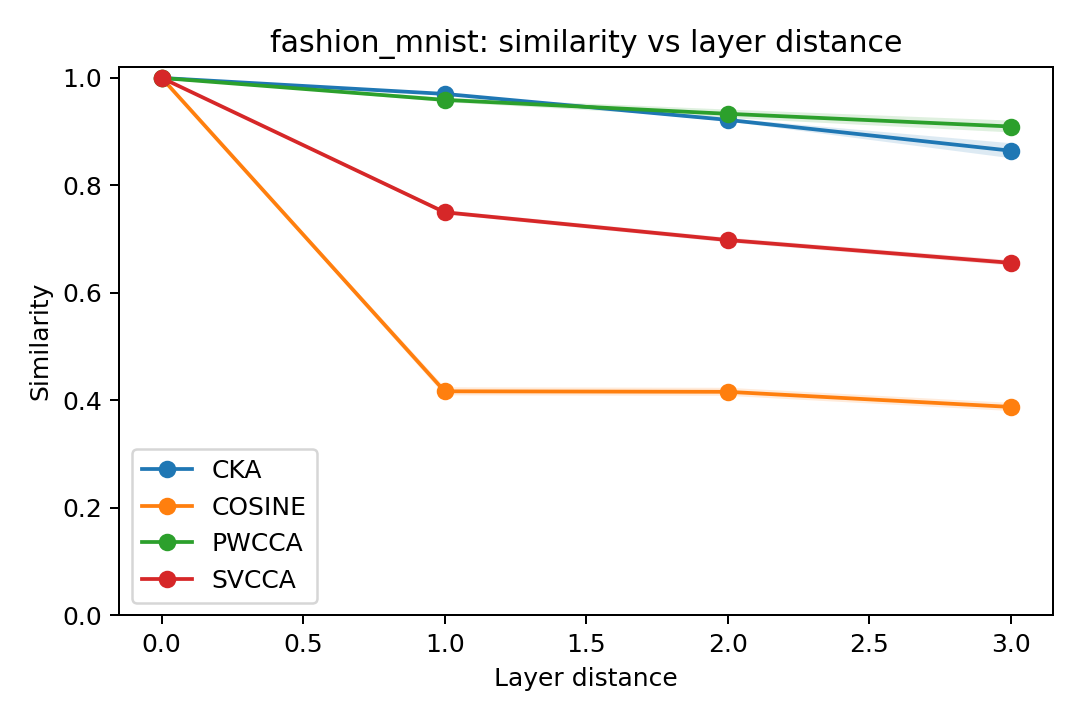
\includegraphics[width=\linewidth]{figures/fashion_mnist_distance_trend.png}
    \end{minipage}\hfill
    \begin{minipage}[t]{0.32\linewidth}
        \centering
        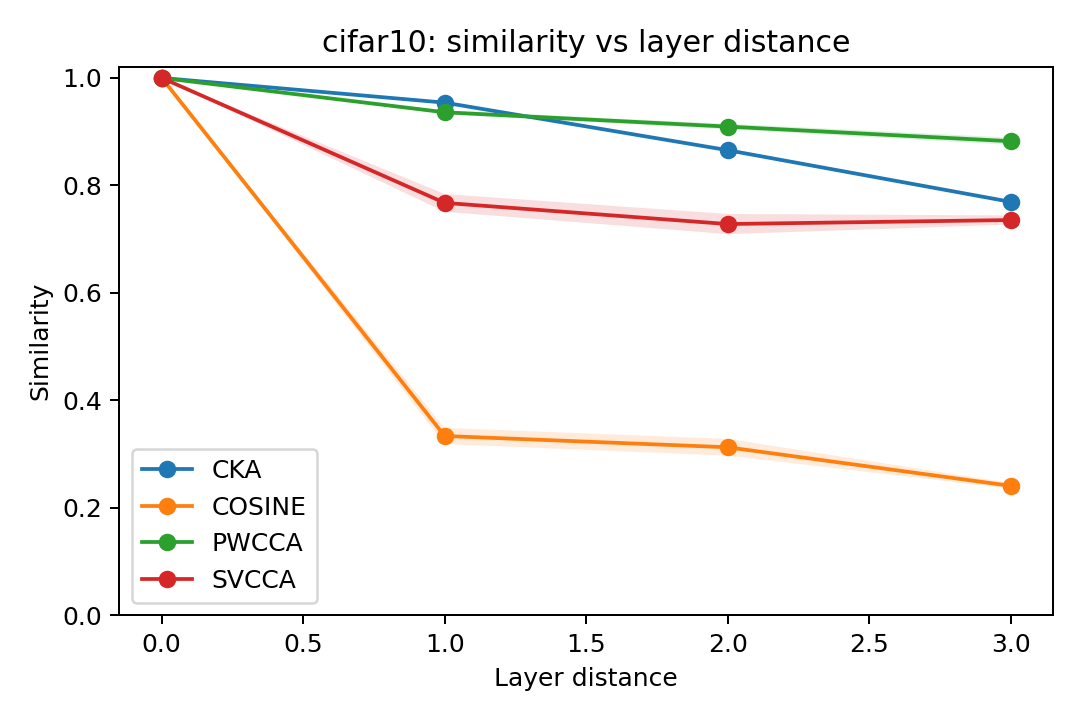
\includegraphics[width=\linewidth]{figures/cifar10_distance_trend.png}
    \end{minipage}
    \caption{Within-model similarity declines with layer distance across all three datasets. The same locality pattern appears with different absolute scales, with the cleanest separation under \cka, \svcca, and \pwcca.}
    \label{fig:distance_trends}
\end{figure}

\para{Within-model locality is the dominant result.} \Tabref{tab:within_model_similarity} shows that adjacent layers are more similar than non-adjacent layers in all 12 dataset-metric comparisons. The effect is strongest and most stable for \cka, \svcca, and \pwcca. For example, on \cifar, adjacent-layer \cka exceeds non-adjacent \cka by $0.1206$ with $p=0.0002$ and Cohen's $d=2.43$. The same qualitative pattern appears on \mnist and \fashionmnist. Cosine similarity is directionally consistent everywhere, but its weaker margins on \mnist and \fashionmnist do not reach $p<0.05$.

\begin{table*}[t]
    \centering
    \small
    \caption{Adjacent-layer versus non-adjacent-layer similarity within the same trained model. Positive differences mean nearby layers are more similar. The largest positive difference for each dataset is in \textbf{bold}.}
    \label{tab:within_model_similarity}
    \resizebox{\textwidth}{!}{%
    \begin{tabular}{@{}llccccc@{}}
        \toprule
        \textsc{Dataset} & \textsc{Metric} & Adjacent Mean & Non-Adjacent Mean & Difference & $p$-value & Cohen's $d$ \\
        \midrule
        \cifar & \cka & \textbf{0.9540} & 0.8335 & \textbf{0.1206} & 0.0002 & 2.43 \\
        \cifar & Cosine & 0.3334 & 0.2885 & 0.0449 & 0.0048 & 0.75 \\
        \cifar & \pwcca & 0.9361 & 0.9004 & 0.0357 & 0.0002 & 1.99 \\
        \cifar & \svcca & 0.7674 & 0.7305 & 0.0369 & 0.0322 & 0.56 \\
        \midrule
        \fashionmnist & \cka & \textbf{0.9703} & 0.9028 & \textbf{0.0674} & 0.0002 & 2.09 \\
        \fashionmnist & Cosine & 0.4166 & 0.4063 & 0.0103 & 0.2280 & 0.30 \\
        \fashionmnist & \pwcca & 0.9591 & 0.9254 & 0.0338 & 0.0002 & 1.23 \\
        \fashionmnist & \svcca & 0.7499 & 0.6841 & 0.0658 & 0.0002 & 2.37 \\
        \midrule
        \mnist & \cka & 0.9793 & 0.9253 & 0.0540 & 0.0002 & 1.85 \\
        \mnist & Cosine & 0.4780 & 0.4636 & 0.0144 & 0.0634 & 0.46 \\
        \mnist & \pwcca & 0.9400 & 0.9161 & 0.0239 & 0.0002 & 1.22 \\
        \mnist & \svcca & \textbf{0.7271} & 0.6591 & \textbf{0.0680} & 0.0002 & 3.18 \\
        \bottomrule
    \end{tabular}%
    }
\end{table*}


\para{Cross-seed layer recurrence is weaker.} \Tabref{tab:cross_seed_similarity} reports same-depth versus off-depth similarity across random seeds. Here the story is mixed: 8 of 12 comparisons favor same-depth alignment, but only 5 are statistically significant. \cka remains the most consistent metric, showing positive and significant same-depth gaps on all three datasets. By contrast, cosine is inconsistent, and both \pwcca and \svcca become weak or negative on \cifar. This means that the claim ``layers are comparable'' is empirically stronger within a single model than across independent initializations.

\begin{table*}[t]
    \centering
    \small
    \caption{Same-depth versus off-depth similarity across random seeds. Positive differences mean the same hidden depth recurs across seeds more strongly than mismatched depths. The strongest positive difference for each dataset is in \textbf{bold}.}
    \label{tab:cross_seed_similarity}
    \resizebox{\textwidth}{!}{%
    \begin{tabular}{@{}llccccc@{}}
        \toprule
        \textsc{Dataset} & \textsc{Metric} & Same-Depth Mean & Off-Depth Mean & Difference & $p$-value & Cohen's $d$ \\
        \midrule
        \cifar & \cka & 0.9359 & 0.8576 & \textbf{0.0783} & 0.0008 & 1.41 \\
        \cifar & Cosine & 0.3211 & 0.3020 & 0.0191 & 0.4993 & 0.19 \\
        \cifar & \pwcca & 0.8878 & 0.8887 & -0.0010 & 0.6237 & -0.14 \\
        \cifar & \svcca & 0.6715 & 0.7018 & -0.0303 & 0.1194 & -0.48 \\
        \midrule
        \fashionmnist & \cka & 0.9160 & 0.8777 & \textbf{0.0383} & 0.0378 & 0.73 \\
        \fashionmnist & Cosine & 0.4051 & 0.4137 & -0.0086 & 0.4265 & -0.24 \\
        \fashionmnist & \pwcca & 0.9411 & 0.9254 & 0.0158 & 0.1400 & 0.47 \\
        \fashionmnist & \svcca & 0.6954 & 0.6761 & 0.0193 & 0.0018 & 0.87 \\
        \midrule
        \mnist & \cka & 0.9560 & 0.9234 & \textbf{0.0326} & 0.0014 & 0.84 \\
        \mnist & Cosine & 0.4562 & 0.4696 & -0.0134 & 0.4579 & -0.20 \\
        \mnist & \pwcca & 0.9166 & 0.9078 & 0.0089 & 0.3583 & 0.26 \\
        \mnist & \svcca & 0.6818 & 0.6568 & 0.0250 & 0.0014 & 0.98 \\
        \bottomrule
    \end{tabular}%
    }
\end{table*}


\begin{figure}[t]
    \centering
    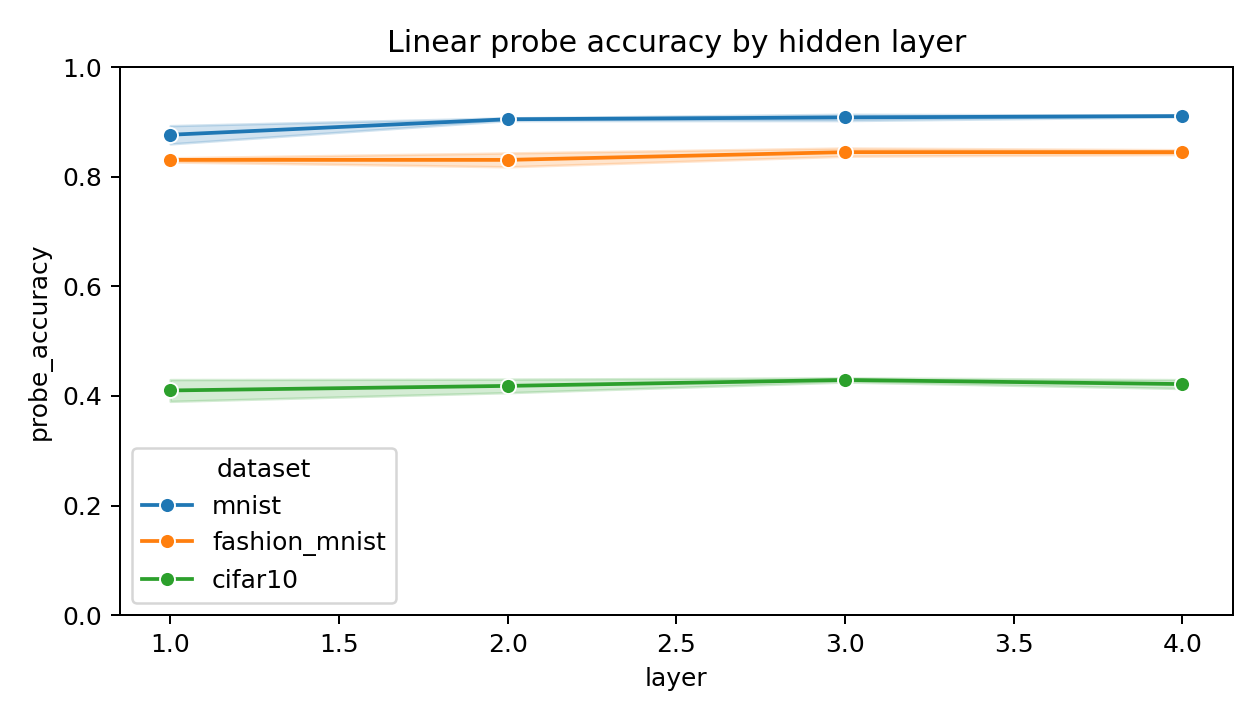
\includegraphics[width=0.78\linewidth]{figures/probe_accuracy_by_layer.png}
    \caption{Linear probe accuracy by hidden layer. Later layers usually improve decodable task information, although the strongest gain on \cifar appears at layer 3 rather than layer 4.}
    \label{fig:probe_accuracy}
\end{figure}

\para{Later layers improve linear decodability.} \Figref{fig:probe_accuracy} complements the geometric results with a task-information view. On \mnist, mean probe accuracy rises from $0.8767$ at layer 1 to {\bf $0.9108$} at layer 4. On \fashionmnist, the best mean accuracy is {\bf $0.8450$} at layers 3 and 4, up from $0.8308$ at layer 1. On \cifar, the best layer is layer 3 with {\bf $0.4292$}, compared with $0.4100$ at layer 1. These gains are modest compared with the overall class difficulty, but they are consistent with a refinement view of depth: later layers improve linearly decodable information while still remaining similar to earlier layers.

\para{Ablation by metric.} The comparison across metrics is itself an informative ablation. \cka, \svcca, and \pwcca all support the progressive-transformation picture within models, while cosine provides the same direction with less stability. Across seeds, only \cka remains consistently positive across datasets. This pattern suggests that metric choice is not a cosmetic decision; it changes how strongly one should believe claims about recurring layer roles across training runs.
